\documentclass[a4paper,11pt]{article}
\usepackage[utf8]{inputenc}
\usepackage[czech]{babel}
\usepackage[left=2cm,top=3cm,text={17cm,24cm}]{geometry}
\usepackage{graphicx}
\usepackage{listings}
\usepackage{url}
\usepackage{xr}
\externaldocument{../manual/manual}
%Konfigurace výpisů kódu
%\lstset{basicstyle=\ttfamily,breaklines=true}
%\lstset{frame=single}

\title{Konfigurace a analýza přenosů VoIP\\
{\bf\large ISA - Laboratorní cvičení č.4}}

\author{Vysoké učení technické v Brně}

\date{\url{https://github.com/nesfit/ISA/tree/master/lab4-voip}}

\begin{document}

{\let\newpage\relax\maketitle}
\section*{Cíl laboratorního cvičení}
\begin{itemize}
  \item Seznámit se s komunikací IP telefonie a signalizačním protokolem SIP.
  \item Nakonfigurovat klienta SIP pro komunikaci VoIP typu peer-to-peer.
  \item Nakonfigurovat klienta SIP pro komunikaci VoIP přes ústřednu. Analyzovat průběh komunikace.
\end{itemize}

\section*{Obecné pokyny}
\begin{itemize}
  \item Vypněte si mobily a uschovejte do tašek. Není dovoleno používat mobily během výuky. 
  \item Zkontrolujte připojení sluchátek s mikrofonem k počítači. 
  \item Přihlašte se do operačního systému MS Windows (F1) jako uživatel {\tt user} s heslem {\tt user4lab}.
%  \item Další informace k IP telefonii a protokolu SIP najdete v laboratorním manuálu, kapitola \ref{sip}. 
\end{itemize}
\vspace{-5mm}

\section{Komunikace VoIP typu peer-to-peer (práce ve dvojicích)}
V této úloze budeme konfigurovat klienta SIP pro komunikaci se svým sousedem bez použití ústředny (spojení typu peer-to-peer). Součástí úlohy je také odchycení komunikace a její analýza. Další informace k IP telefonii a protokolu SIP najdete v laboratorním manuálu, kapitola \ref{sip}. 
%\enlargethispage
\begin{enumerate}
  \item Spusťte aplikaci Jitsi.
    %\footnote{Pokud aplikace není na počítači nainstalovaná, stáhněte ji z \url{https://desktop.jitsi.org/Main/Download.html} a nainstalujte na lokální počítači. Zvolte distribuci Jitsi Desktop Stable pro MS Windows.}
    Povolte přístup přes Windows Firewall, pokud bude vyžadován. Zrušte úvodní dialog. Aplikace běží na pozadí, vyvoláte ji přes ikonu na stavové řádce a položku Show. 
    \item V menu {\tt Tools} $\rightarrow$ {\tt Options} $\rightarrow$ {\tt Accounts} vytvořte nový účet. V poli {\tt Network} zvolte možnost {\tt SIP}. Jako {\tt SIP id} použijte své přihlašovací jméno, {\tt např. xlogin00}, heslo nezadávejte.
    \item Stiskněte tlačítko {\tt Advanced} a v záložce {\tt Security} vypněte podporu šifrování.
    \begin{figure}[h]
    	\centering
    	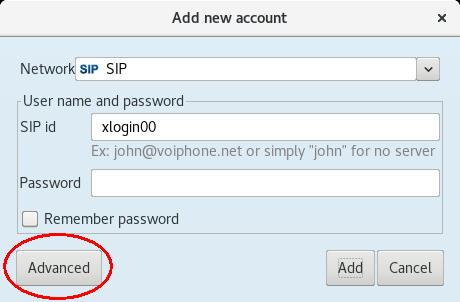
\includegraphics[scale=0.45]{img/account_p2p-b.png}
%    	\caption{Nastavení účtu SIP.}
%    	\label{fig:sip_account}
    \end{figure}

    \item Tlačítky {\tt Next} a {\tt Sign in} vytvoříte nový účet. V seznamu účtů  uvidíte účet s vaším jménem a typem {\it RegistrarLess SIP}, pomocí kterého budete komunikovat přímo s volaným bez registrace na serveru SIP.
    \item Spusťte síťový analyzátor Wireshark a začněte odchytávat pakety na aktivním síťovém rozhraní.
    \item Nastavte display filter tak, aby zobrazoval protokoly SIP a RTP.
    \item V hlavním okně programu Jitsi zadejte do pole {\it Enter name or number} IP adresu vašeho souseda, např. 10.10.10.123.
    \item Zavolejte sousedovi stisknutím tlačítka {\tt sluchátko}. Vyzkoušejte, zda se navzájem slyšíte, a po chvíli hovor ukončete.
      
     {\small Poznámka: V případě problémů se zvukem zkontrolujte, zda není v operačním systému ztlumen mikrofon či audio výstup, případně ověřte nastavení zvukových zařízení v aplikaci Jitsi, menu Tools $\rightarrow$ Options $\rightarrow$ Audio. Zvolený {\tt Audio system} by měl být {\tt WASAPI}, {\tt Audio In} nastavené na hodnotu {\tt Microphone} a {\tt Audio Out} na hodnotu {\tt Headphone}.}
 
   \item Proveďte analýzu navázaného spojení ve Wiresharku. Využijte menu {\tt Telephony $\rightarrow$ VoIP Calls}, kde uvidíte jednotlivé zaznamenané hovory. Vyberte příslušný hovor a zobrazte jeho průběh volbou {\tt Flow}.  Můžete také přehrát zachycený audio přenos tlačítkem {\tt Play Streams}.
     
    \item Do protokolu zakreslete průběh komunikace SIP a RTP mezi oběma klienty. Doplňte IP adresy a porty použité pro signalizaci a transport hlasových dat. Analýzou příkazu INVITE zjistíte seznam podporovaných kodeků na straně volajícího. Nalezené informace zapište do protokolu a uveďte, který kodek byl vybrán pro komunikaci. 

      {\small
      Poznámka: Názvy a čísla podporovaných kodeků si strany vymění protokolem SDP, který je zapouzdřen v těle příkazů {\tt INVITE} a {\tt OK}, viz následující obrázek.
\begin{figure}[h!]
  \centering
  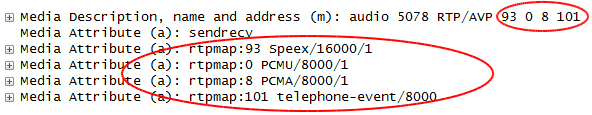
\includegraphics[scale=0.65]{img/3a.png}
\end{figure}

\noindent Informace o vybraném kodeku získáte z hlavičky paketu RTP {\tt Payload type}.
\begin{figure}[h!]
  \centering
  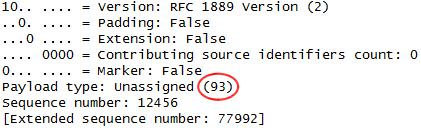
\includegraphics[scale=0.65]{img/3b.png}
\end{figure}
      }
  \item Po ukončení analýzy zrušte v aplikaci Jitsi vámi vytvořený účet, viz menu {\tt Tools} $\rightarrow$ {\tt Options} $\rightarrow$ {\tt Accounts} $\rightarrow$ {\tt Delete}. 
\end{enumerate}


\section{Komunikace VoIP přes ústřednu SIP (práce ve dvojicích)}
V další části cvičení budeme pracovat v aplikaci Jitsi s novým účtem, který vytvoříme v doméně VoIP {\tt isa-lab.cz}. Jméno vašeho účtu (SIP ID) bude {\tt userXX@isa-lab.cz}, heslo {\tt hesloXX} a vaše telefonní číslo {\tt 10XX}, kde {\it XX} je číslo Vašeho počítače. Konfiguraci provedete následujícími kroky: 

\subsection{Registrace VoIP klienta na ústředně}
\begin{enumerate}
    \item Spusťte znovu zachytávání paketů v aplikaci Wireshark.
    \item Vraťte se do hlavního okna aplikace Jitsi a otevřete menu {\tt Tools} $\rightarrow$ {\tt Options} $\rightarrow$ {\tt Accounts}.
    \item Vytvořte nový účet. V poli {\tt Network} vyberte opět možnost {\tt SIP}. Tlačítkem {\tt Advanced} otevřete pokročilou konfiguraci.
    \item V poli {\tt SIP id} nastavte hodnotu {\tt userXX@isa-lab.cz}, heslo {\tt hesloXX}, kde {\tt XX} je číslo vašeho počítače. Do pole {\tt Display name} zadejte své jméno a příjmení (bez diakritiky), viz obrázek \ref{fig:registration1}.
      \begin{figure}[h!]
        \centering
        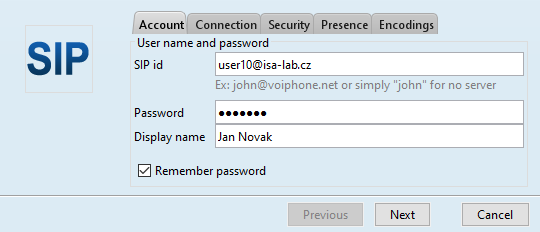
\includegraphics[scale=0.7]{img/jitsi-registration1c.png}
        \caption{Vytvoření účtu.}
        \label{fig:registration1}
      \end{figure}
      
    \item V záložce {\tt Connection} nastavte v políčku {\tt Proxy} IP adresu serveru SIP na hodnotu {\tt 10.10.10.222}.
      Číslo portu zadejte {\tt 5060}, viz obrázek č. \ref{fig:registration2}. 
      \begin{figure}[h!]
        \centering
        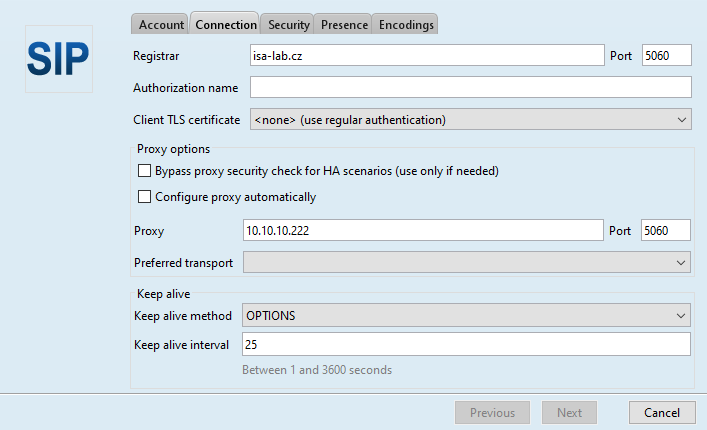
\includegraphics[scale=0.6]{img/jitsi-registration2b.png}
        \caption{Konfigurace adresy ústředny.}
        \label{fig:registration2}
      \end{figure}
    \item Tlačítkem {\tt Next} a {\tt Sign in} dokončíte registraci na ústředně.
    \item  Pokud jste vše nastavili správně, v seznamu účtů v menu {\tt Tools} $\rightarrow$ {\tt Options} uvidíte účet ve stavu {\tt SIP Online}. {\it V případě neúspěchu účet odeberte a znovu přidejte. Pokud ani toto nepomůže, ukončete Jitsi a postupujte znovu od kroku 1, případně konzultujte problém se cvičícím.}
    \item Odhlašte se od ústředny nastavením stavu na hodnotu {\tt Offline}. 
    \item V programu Wireshark analyzujte průběh přihlášení k ústředně a odhlášení. Využijte menu {\tt Telephone} $\rightarrow$ {\tt SIP Flows}. Zaměřte se na pakety s příkazem {\tt REGISTER} a příslušné odpovědi.

      {\small Zprávy typu {\tt PUBLISH, SUBSCRIBE, OPTIONS} můžete ignorovat. Tyto správy slouží k přenosu dodatečných informací o nastavení klienta a my je nebudeme v této laboratoři používat.}
    \item Do protokolu zakreslete průběh registrace. Z hlavičky SIP (položky {\em From, To, Contact, User-Agent, Server, Expires}) určete logickou adresu uživatele (User URI), adresu připojení (Device URI), jméno a verzi klienta SIP, jméno a verzi serveru SIP a maximální dobu přihlášení. Dbejte na správný formát SIP adres.
    \item Zjistěte, čím se liší obsah paketu {\tt REGISTER} při přihlášení a odhlášení uživatele.
\end{enumerate}

\subsection{Analýza hovoru přes ústřednu}
\begin{enumerate}
  \item Znovu se zaregistrujte k ústředně, tj. přepněte účet do stavu {\tt Online}.
  \item Otestujte spojení zavoláním na testovací linku {\tt 123}. V případě správného nastavení systém přehraje automatickou odopověď. 
    \item Obnovte zachytávání paketů v aplikaci Wireshark.
    \item Zavolejte svému sousedovi. V hlavním okně Jitsi zadejte telefonní číslo Vašeho souseda ve formátu {\tt 10XX}, kde {\it XX} je číslo počítače.

    {\small Poznámka: každý z dvojice si zkusí navázat své spojení k sousedovi, které pak bude analyzovat.}
    \item Analyzujte odchycené pakety ve Wiresharku. Zaměřte se na příkazy {\tt INVITE}, {\tt OK} a {\tt ACK}. Z hlaviček {\it From} a {\it Contact} určete hodnoty User URI a Device URI volajícího i volaného. Statistiky přenosu hlasových dat najdete v menu {\tt Telephony} $\rightarrow$ {\tt RTP Streams}. 
    \item Z protokolu SDP určete IP adresu a port pro přenos hlasových dat na straně volajícího i volaného. Zjistěte, jaký kodek byl použitý pro analyzovaný hovor. 
    \item Průběh spojení zakreslete do protokolu a zapište požadované hodnoty.

      {\small Poznámka: každý student zakreslí komunikaci ze svého pohledu, kdy volal sousedovi.}
\end{enumerate}

\subsection{Telefonování přes ústřednu do jiné domény VoIP}
\begin{enumerate}
    \item Na telefonu zvolte telefonní číslo na linku VUT s číslem 54114 1046.
    \item Oznamte telefonicky svému vyučujícímu, že jste práci úspěšně ukončili, a odevzdejte protokol. 
    \item Podle pokynů vyučujícího opravte případné chyby a nepřesnosti v protokolu. 
\end{enumerate}

\section{Ukončení práce v laboratoři}
\begin{itemize}
  %  \item Počítač vypněte spuštěním skriptu {\tt /root/isa4/clean} (jako uživatel {\bf root}).
  \item Zrušte všechny účty vytvořené v aplikaci Jitsi. Ukončete aplikaci pomocí menu {\tt File} $\rightarrow$ {\tt Quit}.
  \item Vypněte počítač. Stočená sluchátka uložte na skříň svého počítače.
\end{itemize}
\end{document}
